\chapter{Meteorological quantities} \label{chap:meteo}
\renewcommand{\tabdir}{chapters/part_processes/meteo/tab}
\renewcommand{\figdir}{chapters/part_processes/meteo/fig}



\section{Introduction} \label{sec:meteo:intro}

In this chapter important meteorological quantities and relationships shall be introduced and described. These are mostly used for the calculation of evapotranspiration (\chapref{chap:et}) and the energy balance based snow simulation (\chapref{chap:snow}).

To directly include the functions and constants into your self-defined model code add \verb!meteo/meteo.h! and \verb!meteo/meteo_const.h! to your auxiliary source code file \verb!userCode_*_aux.cpp!.


\section{Important constants} \label{sec:meteo:constants}
\tabref{tab:meteo:constants} lists all important (hydro-) meteorological, mathematical, and physical constants used in ECHSE with their respective symbols used in this manual, identifiers in the source code, numerical values (precision shown as implemented in ECHSE), units, a short explanation, and a reference.

\begin{table*}
\caption{Constants defined and used in ECHSE.  \label{tab:meteo:constants}}
\begin{tabular}{|p{0.06\textwidth}p{0.13\textwidth}p{0.14\textwidth}p{0.08\textwidth}p{0.24\textwidth}p{0.2\textwidth}|}  \hline
\rowcolor[gray]{0.9}
Symbol & Identifier & Value & Unit & Explanation & Reference \\ \hline
$T_{deg\_K}$ & \verb!T_DEG_K! & \num{273.15} & -- & Conversion term [\celsius] to [K] and vice versa & Any textbook\\
\stefanBoltzmann & \verb!SIGMA! & \num{5.670373e-8} & \si[per-mode=fraction]{\watt\per\metre\squared\per\kelvin\tothe{4}} & Stefan-Boltzmann constant; respect units! & Any textbook\\
$\pi$ & \verb!Pi! & \seqsplit{3.141592653589793} & -- & Pi number & Any textbook\\
\solarConstant & \verb!SOLAR_C! & \num{1360.8} & \si[per-mode=fraction]{\watt\per\metre\squared} & Solar constant; respect units! & \vspace{-\topsep}{\citet{Kopp2011}} (new, revised value!)\\
\molMassDryAir & \verb!M_DA! & \num{28.96546e-03} & \si[per-mode=fraction]{\kilo\gram\per\mole} & Molar mass of dry air & \vspace{-\topsep}\cite{Picard2008}\\
\molMassWater & \verb!M_W! & \num{18.01528e-03} & \si[per-mode=fraction]{\kilo\gram\per\mole} & Molar mass of water & \vspace{-\topsep}\cite{Picard2008}\\
\molGasConst & \verb!R! & \num{8.314} & \si[per-mode=fraction]{\joule\per\mole\per\kelvin} & Molar gas constant & \vspace{-\topsep}\citet{Mohr2005}\\
\karmanConst & \verb!KARMAN! & \num{0.41} & -- & Von K\'arm\'an constant; range of 0.36 to 0.43, 0.41 frequently used in textbooks etc. & \vspace{-\topsep}\citet{Neitsch2011}\\
\specHeatAir & \verb!SPHEATMOIST! & \num{1012} & \si[per-mode=fraction]{\joule\per\kilo\gram\per\kelvin} & Specific heat of moist air under typical room conditions & \url{https://en.wikipedia.org/wiki/Heat_capacity}\\
\hline
\end{tabular}
\end{table*}


\section{Hydro-meteorological quantities}

\subsection{Atmospheric pressure -- \airPressure} \label{sec:meteo:apress}
If no values of atmospheric pressure are given it is possible to assess it from elevation above sea level of your location using the common \emph{barometric formula}. Assuming a temperature lapse rate of \SI{-0.0065}{\kelvin\per\metre}, standard pressure at sea level (\SI{1013.25}{\hecto\pascal}), a temperature of \SI{20}{\degreeCelsius} at sea level, and the air behaving as an ideal gas one obtains the simplified formula as implemented in ECHSE calculating the air pressure (\airPressure{} in [\si{\hecto\pascal}]) at altitude above sea level ($h$, \verb!elev! in [\si{\metre}]) (for derivation see, e.g., \url{https://en.wikipedia.org/wiki/Barometric_formula}):

\begin{equation} \label{eqn:meteo:apress}
  \airPressure{} = 1013.25 \cdot \left[ 1 - \frac{0.0065 \cdot h}{293} \right]^{5.255}
\end{equation}

\noindent
Usage:
\verb!apress_simple(elev)!

Please note that this is only a rough estimation of atmospheric pressure which should only be used if your target variable (e.g. evapotranspiration) is not very sensitive to pressure values!



\subsection{Saturation vapor pressure -- \satVaporPressure} \label{sec:meteo:satvappress}
To calculate saturation vapor pressure a number of different approaches exist using air temperature as dependent variable and assuming standard atmospheric conditions. However, \figref{fig:meteo:satVapPress} shows that the differences between four tested methods are negligible. In ECHSE the \emph{Magnus formula} (sometimes also called \emph{Magnus-Tetens} or \emph{August-Roche-Magnus} formula) as given by \citet{Dyck1995} is implemented whereas separate approaches can be selected for calculations of water and ice surfaces, respectively.\\

\noindent
Over water:

\begin{equation} \label{eqn:meteo:satVapPressWater}
\satVaporPressureWater{} = 6.11 \cdot 10^{\frac{7.5 \cdot \airtemp{}}{273.3 + \airtemp{}}}
\end{equation}

\noindent
Usage:
\verb!satVapPress_overWater(temp)!\\

\noindent
Over ice:

\begin{equation} \label{eqn:meteo:satVapPressIce}
\satVaporPressureIce{} = 6.11 \cdot 10^{\frac{9.5 \cdot \airtemp{}}{265.5 + \airtemp{}}}
\end{equation}

\noindent
Usage:
\verb!satVapPress_overIce(temp)!\\

\satVaporPressureWater{} and \satVaporPressureIce{} are given in [\si{\hecto\pascal}] and air temperature \airtemp{} (\verb!temp!) in [\si{\degreeCelsius}] is used.

\begin{figure}
  \centering
  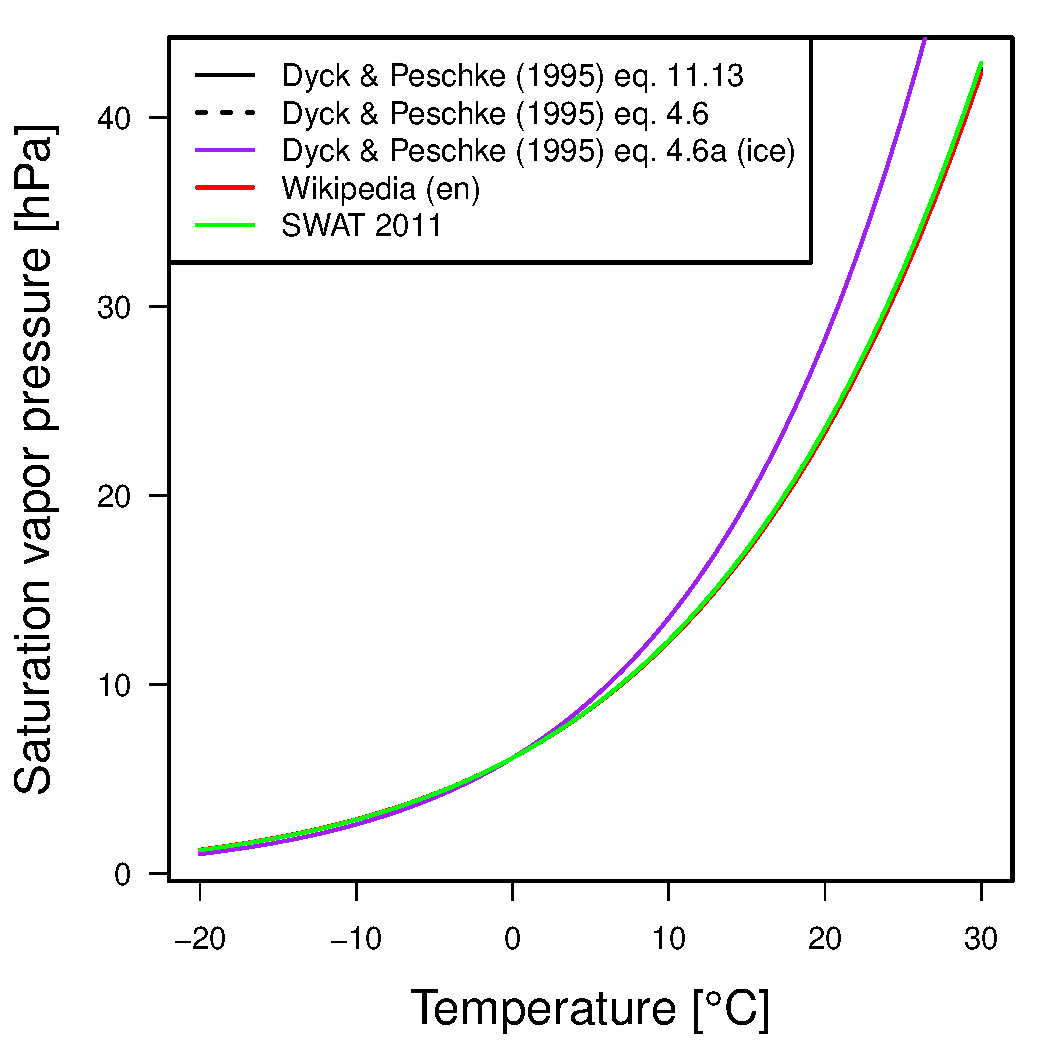
\includegraphics[width=\columnwidth]{\figdir/compare_satVapPress_formulas.ps}
  \caption{Comparison of different approaches for the calculation of saturated water vapor pressure obtained from \citet{Dyck1995, Neitsch2011}, and \url{https://en.wikipedia.org/wiki/Clausius-Clapeyron_relation}. \label{fig:meteo:satVapPress}}
\end{figure}


\subsection{Vapor pressure -- \vaporPressure} \label{sec:meteo:vappress}
As the relative humidity \relHumidity{} (\verb!relhum!) of air is defined as the proportion of actual water vapor pressure \vaporPressure{} to saturated water vapor pressure \satVaporPressure{} (both in [\si{\hecto\pascal}]), the former can be easily derived from measurements of air temperature \airtemp{} (\verb!temp!; in [\si{\degreeCelsius}] to estimate \satVaporPressure{}) and \relHumidity{} in [\si{\percent}]:

\begin{equation} \label{eqn:meteo:vapPress}
\vaporPressure{} = \frac{\satVaporPressure{(\airtemp{})} \cdot \relHumidity{}}{100}
\end{equation}

\noindent
Usage:\\
\verb!vapPress_overWater(temp, relhum)!\\
\verb!vapPress_overIce(temp, relhum)!


\subsection{Vapor pressure deficit -- \vaporPressureDeficit} \label{sec:meteo:vappressdef}
In ECHSE water vapor pressure deficit in [\si{\hecto\pascal}], i.e. $\satVaporPressure{(\airtemp{})} - \vaporPressure{}$ (cf. \secsref{sec:meteo:satvappress} \ref{sec:meteo:vappress}), can by directly computed from air temperature (\airtemp{}, \verb!temp! in [\si{\degreeCelsius}]) and relative humidity (\relHumidity{}, \verb!relhum! in [\si{\percent}]).

\noindent
Usage:\\
\verb!vapPressDeficit_overWater(temp, relhum)!\\
\verb!vapPressDeficit_overIce(temp, relhum)!


\subsection{Slope of the saturation vapor pressure curve -- \slopeSatVapCurve} \label{sec:meteo:slopevappress}
The slope of the saturation vapor pressure temperature curve (\slopeSatVapCurve{} in [\si{\hecto\pascal\per\kelvin}]; in a more general sense also known as \emph{Clausius-Clapeyron} relation) is derived by differentiation of the saturation vapor pressure \satVaporPressure{} with respect to air temperature \airtemp{} (\verb!temp!). \citet{Dyck1995} derived the following equation by differentiation of the \emph{Magnus formula} (cf. \secref{sec:meteo:satvappress}) which is implemented in ECHSE (\airtemp{} in [\si{\degreeCelsius}]):

\begin{equation} \label{eqn:meteo:slopeSatVapCurve}
\slopeSatVapCurve{} = \frac{4098 \cdot \satVaporPressure{(\airtemp{})}}{\left( 273.3 + \airtemp{} \right)^2}
\end{equation}

\noindent
Usage:
\verb!slopeSatVapPress(temp)!\\

Note that herein the temperature dependence of latent heat of evaporation of water is neglected which should, however, be sufficient within the general purpose of evapotranspiration calculation (see Wikipedia for more information: \url{https://en.wikipedia.org/wiki/Clausius-Clapeyron_relation}).


\subsection{Dew point temperature -- \dewpointTemperature} \label{sec:meteo:dewtemp}

TODO


\subsection{Specific humidity -- \specHumidity} \label{sec:meteo:spechum}
Specific humidity (\specHumidity{}, dimensionless) is the ratio of mass of water in a parcel of air to the total mass. \citet{Dyck1995} give the following simplified equation depending on vapor pressure (\vaporPressure{}, \verb!vapPress! in [\si{\hecto\pascal}]; cf. \secref{sec:meteo:vappress}) and air pressure (\airPressure{}, \verb!pressAir! in [\si{\hecto\pascal}]; cf. \secref{sec:meteo:apress}) only:

\begin{equation} \label{eqn:meteo:spechum}
\specHumidity{} = \frac{0.622 \cdot \vaporPressure{}}{\airPressure{} - 0.378 \cdot \vaporPressure{}}
\end{equation}

\noindent
Usage:
\verb!specificHumidity(pressAir, vapPress)!\\


\subsection{Latent heat of water evaporation -- \evapHeatWater} \label{sec:meteo:evapheat}
Latent heat of water evaporation, or heat equivalent of water, (\evapHeatWater{} in [\si{\kilo\joule\per\kilo\gram}]) is a function of temperature (\airtemp{}, \verb!temp! in [\si{\degreeCelsius}]) and can be derived from the following empirical formula \citep{Dyck1995}:

\begin{equation} \label{eqn:meteo:evapheat}
\evapHeatWater{} = 2501 - 2.37 \cdot \airtemp{}
\end{equation}

\noindent
Usage:
\verb!latentHeatEvap(temp)!\\

Note that for sublimation and deposition from and into ice a different formula must be used (not yet included in ECHSE).


\subsection{Psychrometric constant -- \psychroConst} \label{sec:meteo:psychro}
The psychrometric constant (\psychroConst{} in [\si{\hecto\pascal\per\kelvin}]) relates the partial pressure of water in the air to temperature. It depends on atmospheric pressure (\airPressure{}, \verb!airpress! in [\si{\hecto\pascal}]) and heat equivalent of water \evapHeatWater{}, which in turn depends on air temperature (\airtemp{}, \verb!temp! in [\si{\degreeCelsius}]; cf. \secref{sec:meteo:evapheat}), as boundary conditions, and the constants ratio of molecular weight of water vapor to that of dry air and specific heat of air at constant pressure. In summarized form, it can be eventually calculated using the following relation \citep{Dyck1995}:

\begin{equation} \label{eqn:meteo:psychro}
\psychroConst{} = 0.016286 \frac{\airPressure{}}{\evapHeatWater{(\airtemp{})}}
\end{equation}

\noindent
Usage:
\verb!psychroConst(temp, airpress)!\\


\subsection{Mole fraction of water vapor -- \moleFracWaterVap} \label{sec:meteo:molefracvap}
The mole fraction of water vapor is a dimensionless number meaning the amount of water vapor in air. Following the definition from the \emph{International Committee for Weights and Measures CIPM-81/91} its realization in ECHSE is:

\begin{multline}\label{eqn:meteo:molefracvap}
\moleFracWaterVap{} = \relHumidity{} \\ 
(\num{1.00062} + \num{3.14e-08} \cdot \airPressure{} + \num{5.6e-07} \cdot \airtemp{}^2) \\
\frac{\satVaporPressure{(\airtemp{})}}{\airPressure{}}
\end{multline}

\noindent
Usage:\\
\verb!moleFrac_waterVap(airpress,temp,relhum)!\\

Where \relHumidity{}/\verb!relhum! means relative humidity in [\si{\percent}], \airPressure{}/\verb!airpress! is air pressure in [\si{\hecto\pascal}], and \satVaporPressure{} is saturation vapor pressure in [\si{\hecto\pascal}] depending on air temperature (\airtemp{}, \verb!temp! in [\si{\degreeCelsius}]; cf. \secref{sec:meteo:satvappress}). \textbf{Note} that these units are needed for input, internal conversions are applied that are not shown here.


\subsection{Compressibility factor -- \compressibilityFactor} \label{sec:meteo:compressfac}
The compressibility factor (dimensionless) is used to calculate the density of moist air. The ECHSE implementation follows the definition from the \emph{International Committee for Weights and Measures CIPM-81/91} taking into account air pressure (\airPressure{}, \verb!airpress! in [\si{\hecto\pascal}]), temperature (\airtemp{}, \verb!temp! in [\si{\degreeCelsius}]), and relative humidity (\relHumidity{}, \verb!relhum! in [\si{\percent}]) (\textbf{NOTE:} Units shown are needed for input, internal conversions are applied that are not shown here):

\begin{multline}\label{eqn:meteo:compressfac}
\compressibilityFactor{} = 1 - \frac{\airPressure{}}{T_{deg\_K} + \airtemp{}} \\
[a_0 + a_1 t + a_2 t^2 + (b_0 + b_1 t) \moleFracWaterVap{} + (c_0 + c_1 t) \moleFracWaterVap{}^2 ] \\
+ \frac{\airPressure{}^2}{(T_{deg\_K} + \airtemp{})^2} \cdot (d + e \moleFracWaterVap{}^2)
\end{multline}

\noindent
Usage:
\verb!f_compress(airpress,temp,relhum)!\\

\noindent
Where:
\sisetup{
detect-family,
detect-display-math = true
}
\[ a_0 = \SI{1.58123e-06}{\kelvin\per\pascal} \]
\[ a_1 = \SI{-2.9331e-08}{\per\pascal} \]
\[ a_2 = \SI{1.1043e-10}{\per\kelvin\per\pascal} \]
\[ b_0 = \SI{5.707e-06}{\kelvin\per\pascal} \]
\[ b_1 = \SI{-2.051e-08}{\per\pascal} \]
\[ c_0 = \SI{1.9898e-4}{\kelvin\per\pascal} \]
\[ c_1 = \SI{-2.376e-06}{\per\pascal} \]
\[ d = \SI{1.83e-11}{\kelvin\squared\per\pascal\squared} \]
\[ e = \SI{-0.765e-08}{\kelvin\squared\per\pascal\squared} \]

For \moleFracWaterVap{} see \secref{sec:meteo:molefracvap} and for $T_{deg\_K}$ see \secref{sec:meteo:constants}.


\subsection{Density of moist air -- \densityAirMoist} \label{sec:meteo:densairmoist}
To calculate the density of moist air (\densityAirMoist{} in [\si{\kilo\gram\per\cubic\metre}]) the most recent version of the formula from the \emph{International Committee for Weights and Measures (CIPM)}, published and analyzed by \citet{Picard2008}, is incorporated in ECHSE:

\begin{multline}\label{eqn:meteo:densairmoist}
\densityAirMoist{} = \frac{\airPressure{} \cdot \molMassDryAir{}}{\compressibilityFactor{} \cdot \molGasConst \cdot (T_{deg\_K} + \airtemp{})} \\
\left[ 1 - \moleFracWaterVap{} \left( 1 - \frac{\molMassWater{}}{\molMassDryAir{}} \right) \right]
\end{multline}

\noindent
Usage:\\
\verb!densityMoistAir(airpress,temp,relhum)!\\

Air pressure (\airPressure{}, \verb!airpress! in [\si{\hecto\pascal}]), temperature (\airtemp{}, \verb!temp! in [\si{\degreeCelsius}]), and relative humidity (\relHumidity{}, \verb!relhum! in [\si{\percent}]) have to be given. For derivation of \compressibilityFactor{}, and \moleFracWaterVap{} see \secsref{sec:meteo:compressfac}, and \ref{sec:meteo:molefracvap}, respectively. For the constants \molMassDryAir{}, \molMassWater{}, \molGasConst{}, and $T_{deg\_K}$ see \secref{sec:meteo:constants}.


\section{Astronomical quantities}

\subsection{Solar declination -- \solDecl} \label{sec:meteo:soldecl}
Solar declination (\solDecl{} in [\si{\radian}]) is the angle between the rays of the Sun and a plane of the Earth's equator. It varies roughly between \SI{+23.5}{\degree} on June solstice and \SI{-23.5}{\degree} on December solstice caused by the Earth's axial tilt. In ECHSE incorporated is an approximation as used in the SWAT model \citep{Neitsch2011} which should not be used in cases where high accuracy is needed but which is sufficient for estimation of the energy balance (for which \solDecl{} is basically used in ECHSE):

\begin{equation}\label{eqn:meteo:soldecl}
\solDecl{} = \arcsin \left\{ 0.4 \sin \left[ \frac{2 \pi}{365} (\doy{} - 82) \right] \right\}
\end{equation}

\noindent
Usage:
\verb!sol_decl(doy)!\\

Where \doy{} (\verb!doy!) is the current \emph{Julian day} or \emph{day of the year}.


\subsection{Eccentricity correction factor -- \eccCorr} \label{sec:meteo:eccorr}
The eccentricity correction factor \eccCorr{} (dimensionless) accounts for that the Earth's orbit around the Sun is not a perfect circle but slightly elliptical. ECHSE incorporates a simplified formula following the implementation in the SWAT model \citep{Neitsch2011}:

\begin{equation}\label{eqn:meteo:eccorr}
\eccCorr{} = \left( \frac{r_0}{r} \right)^2 = 1 + 0.033 \cos \left(\frac{2 \pi \doy}{365} \right)
\end{equation}

\noindent
Usage:
\verb!eccorr(doy)!\\

Where $r_0$ is the average and $r$ the distance between Earth and Sun for any day of the year, and \doy{} (\verb!doy!) is the current \emph{Julian day} or \emph{day of the year}. For simplification, day \num{366} at leap years is set to \num{365} as otherwise the above formula would not give a reasonable value. It should thus not be used in cases where high accuracy is needed.


\subsection{Daylight time factor -- \dayTimeFac} \label{sec:meteo:daytimefac}
The daylight time factor \dayTimeFac{} is the approximate hour angle in [\si{\radian}] of sunrise and sunset at a specific location at given latitude (\lat{}, \verb!lat! in [\si{\degree}]) on a specific day of the year (\doy{}, \verb!doy!, dimensionless) following equation 25 of FAO's \emph{Guidelines for computing crop water requirements, Chapter 3: Meteorological data} (\url{http://www.fao.org/docrep/X0490E/x0490e07.htm#calculation\%20procedures}):

\begin{equation}\label{eqn:meteo:daytimefac}
\dayTimeFac{} = \arccos \left[ -tan(\solDecl{(\doy)}) tan(\lat{}) \right]
\end{equation}

\noindent
Usage:
\verb!dayTime_fac(doy, lat)!\\

Where \solDecl{} is the solar declination in [\si{\radian}], cf. \secref{sec:meteo:soldecl}. \textbf{Note} that units shown are needed for input, internal conversions are applied.


\subsection{Extraterrestrial radiation -- \radExtraterr} \label{sec:meteo:radex}
Extraterrestrial radiation \radExtraterr{} in [\si{\watt\per\metre\squared}] is the radiation coming from the Sun and hitting the top of the Earth's atmosphere over a given day of the year (\doy{}, \verb!doy!, dimensionless) at a location of given latitude (\lat{}, \verb!lat! in [\si{\degree}]).

On a \textbf{daily} basis it is calculated by integrating incoming solar radiation from sunrise to sunset. See, e.g., \citet{Neitsch2011} or any textbook for a deviation resulting in the following formula (respect units!):

\begin{multline}\label{eqn:meteo:radex_d}
\radExtraterrDaily{} = \frac{1}{\pi} \cdot \solarConstant{} \cdot \eccCorr{} \\
\left[ \dayTimeFac{} \cdot \sin(\solDecl{}) \cdot \sin(\lat{}) + \cos(\solDecl{}) \cdot \cos(\lat{}) \cdot \sin(\dayTimeFac{}) \right]
\end{multline}

\noindent
Usage:
\verb!rad_extraterr_daily(doy, lat)!\\

For \solarConstant{} see \secref{sec:meteo:constants} and for \eccCorr{}, \dayTimeFac{}, and \solDecl{} see \secsref{sec:meteo:eccorr}, \ref{sec:meteo:daytimefac}, and \ref{eqn:meteo:soldecl}, respectively.

To obtain \textbf{hourly} values the solar time angles at the beginning and the end of the hour of interest have to be respected. Furthermore, a correction for the local time zone has to be applied. Following equations 28 to 33 of FAO's \emph{Guidelines for computing crop water requirements, Chapter 3: Meteorological data} (\url{http://www.fao.org/docrep/X0490E/x0490e07.htm#calculation\%20procedures}) the subsequent relations are implemented in ECHSE:

\noindent
Calculation of the solar time angle $\omega_{mid}$ in [\si{\radian}] at the midpoint of the desired hour of the day $h$ (\verb!hour!, integer number):

\begin{multline}\label{eqn:meteo:radex_h:w_mid}
\omega_{mid} = \frac{\pi}{12} \\
\left\{ \left[ (h + 0.5) + 0.06667 \cdot (L_z - L_m) + S_c \right] - 12 \right\}
\end{multline}

\noindent
with $L_m$ (\verb!L_m!) being the longitutde of the location of interest in decimal degrees west of Greenwich (e.g. Greenwich: \SI{0}{\degree}, New York: \SI{75}{\degree}, Berlin: \SI{346.5}{\degree}), $L_z$ the longitude of the center of the local time zone which is computed internally from the deviation of the local time zone from universal time (UTC) which has to be given as input (\verb!utc_add!, integer value of [\numrange[range-phrase=..]{-12}{14}])\footnote{\textbf{Note} that the value might change over the year in case of \emph{daylight saving time} and thus should be given as time series input rather than just being a fixed parameter!}, and $S_c$ a seasonal correction factor that is computed internally. Using that the solar time angles at begin and end of the hour of interest can be calculated:

\begin{equation}\label{eqn:meteo:radex_h:w_ini_end}
\begin{split}
\omega_{ini} &= \omega_{mid} - \frac{\pi}{24},\\
\omega_{end} &= \omega_{mid} + \frac{\pi}{24}
\end{split}
\end{equation}

\noindent
where, of course, radiation is zero if $\omega_{mid} < -\dayTimeFac{}$ or $\omega_{mid} > \dayTimeFac{}$ (for \dayTimeFac{} see \secref{sec:meteo:daytimefac}), i.e. if the Sun is not shining (note from \eqnref{eqn:meteo:radex_h:w_mid} that the accuracy is $\pm$ half an hour). Eventually, analog to \radExtraterrDaily{}, hourly values of \radExtraterr{} can be obtained:

\begin{multline}\label{eqn:meteo:radex_h}
\radExtraterrHourly{} = \frac{1}{\pi} \cdot \solarConstant{} \cdot \eccCorr{}\\
\big[ (\omega_{end}-\omega_{ini}) \cdot \sin(\solDecl{}) \cdot \sin(\lat{})\\
+ \cos(\solDecl{}) \cdot \cos(\lat{}) \cdot (\sin(\omega_{end})-\sin(\omega_{ini})) \big]
\end{multline}

\noindent
Usage:
\begin{verbatim}
rad_extraterr_hourly(doy,lat,hour,
utc_add,L_m)
\end{verbatim}

\figref{fig:meteo:radex_h} shows example outputs of hourly extraterrestrial radiation computed with \eqnsref{eqn:meteo:radex_h:w_mid} to \ref{eqn:meteo:radex_h} over four specific days of year for Berlin taking \emph{daylight saving time} into account.

\begin{figure}
  \centering
  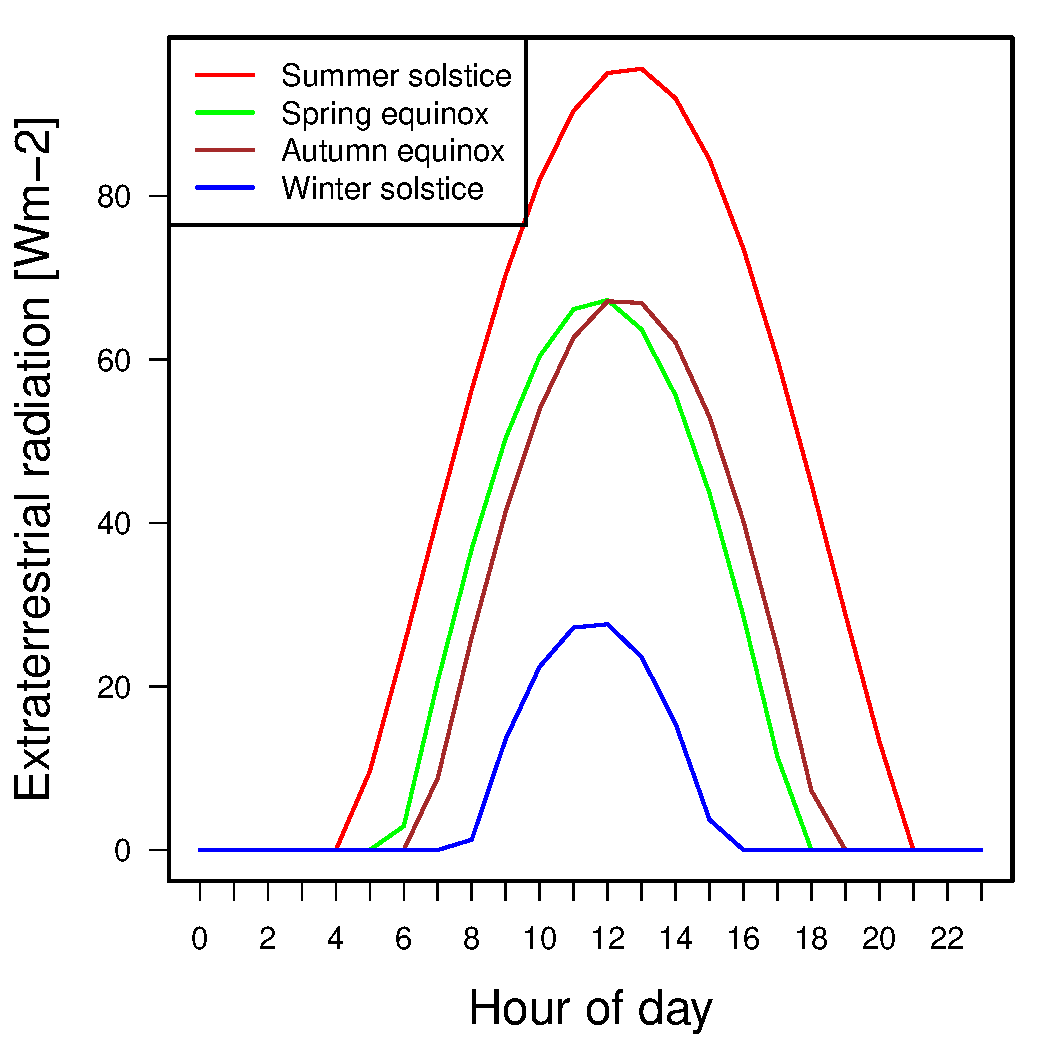
\includegraphics[width=\columnwidth]{\figdir/test_radex_hourly.ps}
  \caption{Hourly extraterrestrial radiation computed using \eqnsref{eqn:meteo:radex_h:w_mid} to \ref{eqn:meteo:radex_h} over four specific days of year (line colors, see legend) for Berlin taking \emph{daylight saving time} into account.\label{fig:meteo:radex_h}}
\end{figure}

\textbf{Note} that units shown are needed for input, internal conversions are applied.


\section{Energy budget}

\subsection{Incoming short-wave radiation -- \radShortwaveIn} \label{sec:meteo:radshort}
Shortwave radiation received by the surface is typically lower than \emph{extraterrestrial radiation} discussed in \secref{sec:meteo:radex} due to processes of absorption, scattering, and reflection in the Earth's atmosphere. It is typically measured at weather stations but can be calculated if no observations are available using the relation of {\AA}ngström (see textbooks, e.g. \citet{Maidment1993}):

\begin{equation}\label{eqn:meteo:radshort}
\radShortwaveIn{} = \left( a_s + b_s \frac{n}{N} \right) \radExtraterr{}
\end{equation}

\noindent
Usage:
\begin{verbatim}
calc_glorad(radex,sundur,cloud,lat
doy,radex_a,radex_b)
\end{verbatim}

\radShortwaveIn{} is computed in [\si{\watt\per\metre\squared}], \radExtraterr{} is extraterrestrial radiation (\verb!radex! in [\si{\watt\per\metre\squared}], cf. \secref{sec:meteo:radex}), $\frac{n}{N}$ is the fraction of measured (\verb!sundur!) to maximum possible sunshine duration, the latter calculated internally from \dayTimeFac{} (cf. \secref{sec:meteo:daytimefac}) which needs the current day of year \verb!doy! and the latitude \verb!lat! of the location of interest in [\si{\degree}] as inputs:

\begin{equation}\label{eqn:meteo:radshort:sundur}
N = \dayTimeFac{} \frac{24}{\pi}
\end{equation}

$a_s$ (\verb!radex_a!) and $b_s$ (\verb!radex_b!) are the {\AA}ngström coefficients. The latter define the fraction of \radExtraterr{} that reaches the surface on completely cloudy ($a_s$) and days of clear sky ($a_s + b_s$), respectively. They can be estimated from measured values (e.g. from a near-by station) or derived from look-up tables (for average climates \citet{Maidment1993} suggests $a_s = \num{0.25}$ and $b_s = \num{0.50}$). Note that measurements of cloudiness (\verb!cloud!) as input to estimate $\frac{n}{N}$ are not yet supported (although the function interface includes it) but planned for the future.

\textbf{Note} that units shown are needed for input, internal conversions are applied.


\subsection{Maximum (clear-sky) incoming short-wave radiation -- \radShortwaveInClearsky} \label{sec:meteo:radshortmax}
The maximum possible incoming short-wave radiation in case of clear sky (\radShortwaveInClearsky{} in [\si{\watt\per\metre\squared}]) is calculated analogue to \radShortwaveIn{} (cf. \secref{sec:meteo:radshort}) assuming full sunshine duration and thus $\frac{n}{N} = \num{1}$:

\begin{equation}\label{eqn:meteo:radshortmax}
\radShortwaveInClearsky{} = \left( a_s + b_s \right) \radExtraterr{}
\end{equation}

\noindent
Usage:\\
\verb!calc_glorad_max(radex,radex_a,radex_b)!


\subsection{Net emissivity -- \emissivity} \label{sec:meteo:emiss}
Emissivity characterizes the effectiveness of a surface in emitting energy as thermal long-wave radiation. In this case the net emissivity between the Earth's surface and the atmosphere is sought which depends on the amount of water in the air and can thus be empirically related to the water vapor pressure (\vaporPressure{} in [\si{\hecto\pascal}]; cf. \secref{sec:meteo:vappress}) \citep{Maidment1993}:

\begin{equation}\label{eqn:meteo:emis_1}
\emissivity{} = a_e + b_e \sqrt{\vaporPressure{}}
\end{equation}

\noindent
Usage:
\verb!net_emiss(temp,relhum,a,b)!\\

The parameters $a_e$ and $b_e$ are in the range of \num{0.34} to \num{0.44} and \num{-0.25} to \num{-0.14}, respectively, whereas for average conditions the values $a_e = \num{0.34}$ and $b_e = \num{-0.14}$ are typically used \citep{Maidment1993}.

If no measurements of relative humidity (\relHumidity{}, \verb!relhum! in [\si{\percent}]) for estimation of \vaporPressure{} are available, \emissivity{} can be as well estimated solely from temperature (\airtemp{}, \verb!temp! in [\si{\degreeCelsius}]) \citep{Maidment1993}:

\begin{equation}\label{eqn:meteo:emis_2}
\emissivity{} = -0.02 + 0.261 \exp(\num{-7.77e-4} \airtemp{}^2)
\end{equation}

\textbf{Note} that units shown are needed for input, internal conversions are applied.


\subsection{Cloudiness correction factor -- \cloudCorrFac} \label{sec:meteo:cloudcorr}
The cloudiness correction factor (\cloudCorrFac{}, dimensionless) is an empirical factor to correct calculations of long-wave radiation at the Earth's surface for cloud cover (cf. \secref{sec:meteo:radnetlong}). It can be calculated from the ratio of actual short-wave radiation (\radShortwaveIn{}, \verb!glorad! in [\si{\watt\per\metre\squared}]) to maximum short-wave radiation at clear sky (\radShortwaveInClearsky{}, \verb!glorad_max! in [\si{\watt\per\metre\squared}]) \citep{Maidment1993}:

\begin{equation}\label{eqn:meteo:cloudcorr}
\cloudCorrFac{} = a_c \frac{\radShortwaveIn{}}{\radShortwaveInClearsky{}} + b_c
\end{equation}

\noindent
Usage:
\verb!f_cloud(glorad,glorad_max,a,b)!\\

The long-wave radiation coefficients for clear skies $a_c$ and $b_c$ should be estimated from local radiation measurements. However, \citet{Maidment1993} suggests $a_c = \num{1.35}$ and $b_c = \num{-0.35}$ for arid areas, and $a_c = \num{1.00}$ and $b_c = \num{0.00}$ for humid areas.


\subsection{Incoming net long-wave radiation -- \netRadiationLong} \label{sec:meteo:radnetlong}
Applying the \emph{law of Stefan-Boltzmann} the incoming net long-wave radiation at the Earth's surface (\netRadiationLong{} in [\si{\watt\per\metre\squared}]) can be calculated from \citep{Maidment1993}:

\begin{equation}\label{eqn:meteo:radnetlong}
\netRadiationLong{} = - \cloudCorrFac{} \emissivity{} \stefanBoltzmann{} (\airtemp{} + T_{deg\_K})^4
\end{equation}

\noindent
Usage:
\begin{verbatim}
net_longrad(temp,relhum,glorad,
glorad_max,emis_a,emis_b,
fcorr_a,fcorr_b)
\end{verbatim}

\netRadiationLong{} is defined positive in direction to the ground, i.e. negative values indicate a net loss, positive values net gain of energy at the Earth's surface. For \cloudCorrFac{} (including the radiation coefficients \verb!fcorr_a! and \verb!facorr_b!) and \emissivity{} (including the emissivity parameter \verb!emis_a! and \verb!emis_b!) see \secsref{sec:meteo:cloudcorr} and \ref{sec:meteo:emiss}, respectively. For \stefanBoltzmann{} and $T_{deg\_K}$ see \secref{sec:meteo:constants}. \airtemp{} (\verb!temp!) is the air temperature in [\si{\degreeCelsius}].


\subsection{Incoming net radiation -- \netRadiation} \label{sec:meteo:radnet}
The total incoming net radiation (\netRadiation{} in [\si{\watt\per\metre\squared}]) is the sum of incoming net long-wave radiation (\netRadiationLong{}, cf. \secref{sec:meteo:radnetlong}) and incoming net short-wave radiation, i.e. the amount of incoming short-wave radiation \radShortwaveIn{} (cf. \secref{sec:meteo:radshort}) absorbed by the ground \citep{Maidment1993}:

\begin{equation}\label{eqn:meteo:radnet}
\netRadiation{} = (1 - \albedo{}) \radShortwaveIn{} + \netRadiationLong{}
\end{equation}

\noindent
Usage:
\begin{verbatim}
net_rad(temp,relhum,glorad,glorad_max,
emis_a,emis_b,fcorr_a,fcorr_b)
\end{verbatim}

Albedo (\albedo{}) is a quantity depending on land cover. It can be derived from local measurements of the radiation balance or from look-up tables. As it might change over the year it is advised to supply it as time series input rather than as a fixed parameter.


\subsection{Soil heat flux -- \heatfluxSoil} \label{sec:meteo:soilflux}
Soil heat flux (\heatfluxSoil{} in [\si{\watt\per\metre\squared}]) is the conduction of heat through the soil. It varies over the day and depends on land-cover conditions. According to textbooks it can be neglected over daily time scales which is generally done in the context of hydrological applications. At sub-daily application, however, it cannot be neglected and is typically defined as a fraction of net radiation \netRadiation{} (\verb!net_rad! in [\si{\watt\per\metre\squared}]). In equations 45 and 46 of FAO's \emph{Guidelines for computing crop water requirements, Chapter 3: Meteorological data} (\url{http://www.fao.org/docrep/X0490E/x0490e07.htm#calculation\%20procedures}) it is suggested to take \SI{10}{\percent} during daylight periods and \SI{50}{\percent} during nighttime, \citet{Shuttleworth1985} arbitrarily set it to \SI{20}{\percent}, and \citet{Guentner2002} identified in a literature study \SI{20}{\percent} during daytime and \SI{70}{\percent} for nighttime periods as appropriate for (semi-)arid conditions with sparse vegetation cover. These approaches are implemented in ECHSE, taking the fraction of \netRadiation{} over daytime (\verb!f_day!) and nighttime (\verb!f_night!), a flag specifying if, at the current time step, it is day ($\verb!daynight! = 1$) or nighttime ($\verb!daynight! = 0$), and the current time step length (\verb!delta_t! in [\si{\second}]) to differentiate between the two approaches as inputs.\\

\noindent
Usage:
\begin{verbatim}
soil_heatflux(net_rad,f_day,f_night,
daynight,delta_t)
\end{verbatim}

For monthly time scales further approaches exist depending on temperature, soil heat conductivity, and effective soil depth (cf. \citet{Maidment1993} or \url{http://www.fao.org/docrep/X0490E/x0490e07.htm#calculation\%20procedures}).
